% Définition paramètres documents

\documentclass[a4paper, 12pt]{report}

\usepackage[utf8]{inputenc} 	%package pour le français sous ubuntu : à vous d'adapter
\usepackage[french]{babel}	%pour le français
\usepackage[T1]{fontenc}	%pour les polices
\usepackage{amsmath}		%pour des maths
\usepackage{amsfonts}		%pour des maths
\usepackage{amssymb}		%pour des maths
\usepackage{graphicx}		%pour les inclusions de graphique
\usepackage{palatino}		%choix personnel de police
\usepackage{lscape}		%si vous voulez des images en paysage
\usepackage{esint}		%pour les triples intégrales
\usepackage[left=2cm, right=2cm, top=2cm, bottom=2cm]{geometry} % choix personnel de marges
\usepackage{hyperref}		%pour les liens croisés à travers le fichier .pdf
\usepackage{fancyhdr}		%pour les marges
\usepackage{float, caption}	%pour le positionnement et légende des images
\usepackage{titlesec}		%pour redéfinir le titre des sections
\usepackage{color}		%pour la couleur dans le code
\usepackage{listings}		%pour mettre du code, plutôt en Annexe
\usepackage{lastpage}		%pour les références aux pages
\usepackage{epic,eepic}		%pour le positionnement de l'image de garde
\usepackage{wrapfig}		%pour les images sur le coté dans le texte
\usepackage{calc,ifthen,xspace}	%pour redéfinir les espaces et distances
\pagestyle{fancy}




\hypersetup{
dvips,
backref=true, %permet d'ajouter des liens dans...
pagebackref=true,%...les bibliographies
hyperindex=true, %ajoute des liens dans les index.
colorlinks=true, %colorise les liens
breaklinks=true, %permet le retour à la ligne dans les liens trop longs
urlcolor= blue, %couleur des hyperliens
linkcolor= black, %couleur des liens internes
bookmarks=blue, %créé des signets pour Acrobat
bookmarksopen=true} 






\definecolor{hellgelb}{rgb}{1,1,0.8} % couleur pour le code
\definecolor{colKeys}{rgb}{0,0,1}
\definecolor{colIdentifier}{rgb}{0,0,0}
\definecolor{colComments}{rgb}{0,0.5,0}
\definecolor{colString}{rgb}{0.62,0.12,0.94}
\definecolor{INSA_GM}{cmyk}{0.6,0,0,0} % et la page de garde
\definecolor{INSA_GRIS}{cmyk}{0.7,0.6,0.5,0.3}
\definecolor{INSA_BLEU}{cmyk}{1,0.9,0.1,0}

%\titleformat{\chapter}[display]%
%	{}
%	{}
%	{0pt}
%	{\Huge\bfseries \thechapter. \quad}
%	{}
\newcommand{\insertrefproj}[1]{}
\newcommand{\refproj}[1]{\renewcommand{\insertrefproj}{\textbf{\color{INSA_GRIS}#1}}}

\fancypagestyle{courant}{%
	\fancyhf{}
    \setlength{\headheight}{27pt}
    \fancyhead[L]{\raisebox{-2mm}{
\includegraphics[width=30mm]{images/insalogo2.png}}}
\fancyhead[C]{}
\fancyhead[R]{\color{INSA_GRIS}\thepage}%\scshape\leftmark}
\fancyfoot[L]{\insertrefproj}
\fancyfoot[R]{}
%\fancyfoot[CE,CO]{\color{INSA_GRIS}\thepage}
\renewcommand{\headrulewidth}{0pt}
\renewcommand{\footrulewidth}{0.2pt}
}

\fancypagestyle{special}{%
  \pagestyle{courant}
  \fancyfoot{}
  %\addtolength{\footskip}{-20pt}
%  \setlength{\footskip}{0pt}
%  \fancyfoot[C]{}
\renewcommand{\footrulewidth}{0pt}
}
% Redefine the plain page style (for chapters and toc)
\fancypagestyle{plain}{%
  \fancyhf{}%
  \pagestyle{courant}
}


\newcommand{\Scilab}{
	\lstset{
	language=Scilab,
	float=hbp,
	basicstyle=\ttfamily\small,
	identifierstyle=\color{colIdentifier},
	keywordstyle=\bf \color{colKeys},
	stringstyle=\color{colString},
	commentstyle=\color{colComments},
	columns=flexible,
	tabsize=5,
	frame=single,
	%frame=shadowbox,
	rulesepcolor=\color[gray]{0.5},
	extendedchars=true,
	showspaces=false,
	showstringspaces=false,
	numbers=left,
	stepnumber=5,
	firstnumber=1,
	numberstyle=\tiny,
	breaklines=true,
	%backgroundcolor=\color{hellgelb},
	captionpos=b,
	}
}

\title{Projet de P6}
\refproj{STPI/P6/20xx - ****}  % Entrer ici la reference du projet
\author{Martin ROSALIE}
\date{}

\begin{document}
%%%%%%%%%%%% Page de Présentation %%%%%%%%%%%%%
\pagenumbering{Alph}
\thispagestyle{empty}
\vspace{4cm}
\begin{picture}(0,0)%(hauteur,largeur)
%\put(-74,-776){\includegraphics[width=210mm]{images/couverture.png}}
	\put(-44,-465){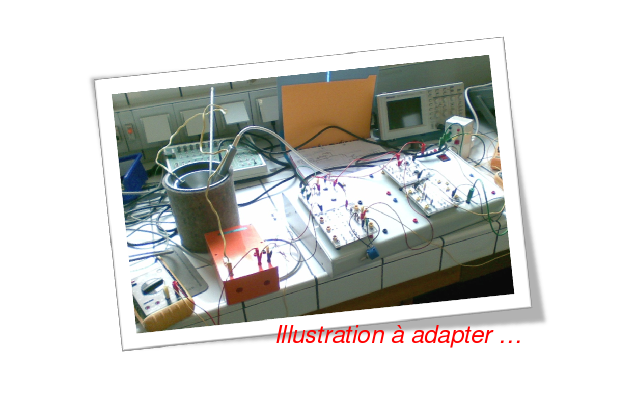
\includegraphics[scale=1]{images/imageGarde.png}}% Illustration à adapter
%\put(-74,-776){\includegraphics[width=210mm]{images/couverture.png}}
  \put(0,-20){
\includegraphics[width=0.4\textwidth]{images/insalogo2.png}}
	\put(240,0){\color{INSA_GM}{\begin{minipage}{12cm}\centering \Large \textbf{Projet de Physique P6}\\\textbf{STPI/P6/20xx-\#\#\#}\end{minipage}}}
\put(-20,-150){\color{INSA_BLEU}{\begin{minipage}{\textwidth}\centering \Huge \textbf{Intitulé du projet}\end{minipage}}}

\newsavebox{\noms}
\savebox{\noms}(300, 300)[tl]{
\put(0,98){\color{INSA_GRIS}{\begin{minipage}{6cm} \textbf{Étudiants :} \end{minipage}}}
\put(0,60){\color{INSA_GRIS}{\begin{minipage}{6cm} Prénom1 NOM1 \\ Prénom3 NOM3 \\ Prénom5 NOM5 \\Prénom7 NOM7 \end{minipage}}}
	\put(185,60){\color{INSA_GRIS}{\begin{minipage}{6cm} Prénom2 NOM2 \\ Prénom4 NOM4 \\ Prénom6 NOM6 \\ Prénom8 NOM8 \end{minipage}}}
	%%\put(-74,-680){\color{INSA_GRIS}\begin{minipage}{6.8cm} \Large \raggedleft Enseignant responsable \\ Prénom NOM

    \put(0,){\color{INSA_GRIS}\begin{minipage}{9cm}   \textbf{Enseignant-responsable du projet :}\\ Prénom NOM
	%\put(-74,-680){\color{INSA_GRIS}\begin{minipage}{6.8cm} \Large \raggedleft Enseignant responsable \\ Prénom NOM
 \end{minipage}}
}

\put(100,-850){\usebox{\noms}}

\end{picture}
%\raggedleft
%%%%%%%% Fin de la page de Présentation %%%%%%
\newpage
\pagenumbering{arabic}
\setcounter{page}{1}
\thispagestyle{empty}
\null %rempli la page de rien
\newpage
\pagestyle{special}



	\textbf{Date de remise du rapport :} XX/XX/20XX\\



	\textbf{Référence du projet:} STPI/P6/20xx – \#\#\# \\

	\textbf{Intitulé du projet :} x \\

	\textbf{Type de projet :} \textit{(expérimental, simulation, veille technologique...)} \\

	\textbf{Objectifs du projet :} \textit{($10$ lignes maximum)}\\ 

	xxx\\


\textbf{Mots-clefs du projet :} \textit{($4$ maximum)} \\ 


	\textit{Si existant} \textbf{Numéro de cahier de laboratoire associé :} XXX

\vfill
%	\textbf{Remerciements :}\\
%
%	xxx\\
\vfill
\begin{center}
  \color{INSA_BLEU}\scshape institut national des sciences appliquées de rouen \\
	Département Sciences et Techniques Pour l'Ingénieur \\
	685 Avenue de l'Université BP 08- 76801 Saint-Etienne-du-Rouvray \\ Tél : 33 2 32 95 66 21 - Fax : 33 2 32 95 66 31
\end{center}
\newpage
\pagestyle{courant} 
	\setcounter{tocdepth}{2}
	\tableofcontents

  
	\chapter*{Notations et Acronymes}		% garde la même mise en page qu'un chapitre mais ne le numérote pas
	\addcontentsline{toc}{chapter}{Notations}	% permet de l'avoir dans le sommaire

\begin{description}
	\item[Notation à définir :] définition
	\item[Acronymes à définir :] acronyme
\end{description}

\newpage
	\chapter*{Introduction}				% garde la même mise en page qu'un chapitre mais ne le numérote pas
	\addcontentsline{toc}{chapter}{Introduction}	% permet de l'avoir dans le sommaire

	\begin{itemize}
	\item Contexte du travail
	\item Objectifs à atteindre pour le projet
	\end{itemize}

	\chapter{Méthodologie, organisation du travail}

	\begin{itemize}
	\item Description de l’organisation adoptée pour le déroulement du travail
	\item Organigramme des tâches réalisées et des étudiants concernés
	\end{itemize}

	\chapter{Travail réalisé et résultats}

		\section{Section}

			\subsection{Sous-section}

				\subsubsection{Sous-sous-section}


\begin{figure}[h]
\centering
\vspace{-0.6cm} 
%\includegraphics[width=0.62\linewidth]{PistonHeatReservoir.pdf}

\includegraphics[width=43mm]{images/insalogo2.png}\captionof{figure}[LogoINSA]{Super Logo}
%\vspace{-2.cm} 
\end{figure}



	Lorem ipsum dolor sit amet, consectetuer adipiscing elit. Sed non risus. Suspendisse lectus tortor, dignissim sit amet, adipiscing nec, ultricies sed, dolor. Cras elementum ultrices diam. Maecenas ligula massa, varius a, semper congue, euismod non, mi. Proin porttitor, orci nec nonummy molestie, enim est eleifend mi, non fermentum diam nisl sit amet erat. Duis semper. Duis arcu massa, scelerisque vitae, consequat in, pretium a, enim. Pellentesque congue. Ut in risus volutpat libero pharetra tempor. Cras vestibulum bibendum augue. Praesent egestas leo in pede. Praesent blandit odio eu enim. Pellentesque sed dui ut augue blandit sodales. Vestibulum ante ipsum primis in faucibus orci luctus et ultrices posuere cubilia Curae; Aliquam nibh. Mauris ac mauris sed pede pellentesque fermentum. Maecenas adipiscing ante non diam sodales hendrerit.\\

%Si vous voulez numéroter les équations faîtes ceci : 
\begin{equation}
	y = a x + b
\end{equation}
%Sinon mettez juste $$ y = ax + b $$

				\subsubsection{Conseils de rédaction}

	Le rapport ne devra pas dépasser un nombre maximum de \textbf{20 pages} (hors annexes). Les informations attendues dans ce rapport sont données ci-dessous. Toutefois, l’organisation et les intitulés des chapitres sont laissés au libre choix des étudiants. La mise en page de ce document est à respecter. 

	\chapter*{Conclusion et perspectives}		% garde la même mise en page qu'un chapitre mais ne le numérote pas
	\addcontentsline{toc}{chapter}{Conclusion et perspectives}% permet de l'avoir dans le sommaire
\begin{itemize}
\item Conclusions sur le travail réalisé
\item Conclusions sur l’apport personnel de cte E.C. projet
\item Perspectives pour la poursuite de ce projet
\end{itemize}

\begin{thebibliography}{9}
	\addcontentsline{toc}{chapter}{Bibliographie}	% permet de l'avoir dans le sommaire

	\bibitem{Livre 01}
		\textsc{Nom}, Prénom
		\textit{Titredu livre },
		Editeur, Année.

	\bibitem{Article 01}
		\textsc{Nom des Auteurs},
		"\textit{Titre de l'article}",
		Titre du journal,
		Volume, pages, année.

	\bibitem{Lien Internet 01}
\textsc{lien Internet},
		\url{http://www.\#\#\#\#}
		(Valide à la date du \#\#/\#\#/201\#)

\end{thebibliography}

\appendix

	\chapter{Documentation technique}

Les annexes ne sont pas obligatoire, les annexes présentées ici le sont à titre indicatif.
	\chapter{Listings des programmes réalisés}
	\chapter{Schémas de montages, \\plans de conception...}
	\chapter{Propositions de sujets de projets \\ (en lien ou pas avec le projet réalisé)}
	\chapter{Mettre du code en annexe}

	Voici comment mettre du code source en annexe. Attention ! Les accents et caractères spéciaux ne sont pas pris en compte pour l'insertion de code.\\

	\Scilab
	\lstinputlisting{code/code.sce}

\end{document}
